\documentclass[manuscript, letterpaper]{aastex6}

\include{gitstuff}
% ----------------------------------- %
% start of AASTeX mods by DWH and DFM %
% ----------------------------------- %

\setlength{\voffset}{0in}
\setlength{\hoffset}{0in}
\setlength{\textwidth}{6in}
\setlength{\textheight}{9in}
\setlength{\headheight}{0ex}
\setlength{\headsep}{\baselinestretch\baselineskip} % this is 2 lines in ``manuscript''
\setlength{\footnotesep}{0in}
\setlength{\topmargin}{-\headsep}
\setlength{\oddsidemargin}{0.25in}
\setlength{\evensidemargin}{0.25in}

\linespread{0.54} % close to 10/13 spacing in ``manuscript''
\setlength{\parindent}{0.54\baselineskip}
\hypersetup{colorlinks = false}
\makeatletter % you know you are living your life wrong when you need to do this
\long\def\frontmatter@title@above{
\vspace*{-\headsep}\vspace*{\headheight}
\noindent\footnotesize
{\noindent\footnotesize\textsc{\@journalinfo}}\par
{\noindent\scriptsize Preprint typeset using \LaTeX\ style AASTeX6
with modifications by DWH and DFM.
}\par\vspace*{-\baselineskip}\vspace*{0.625in}
}%
\long\def\frontmatter@abstractheading{%
\makeaffils
  \vspace*{-\baselineskip}\vspace*{1.5pt}
  \vspace*{0.13189in}
 \begingroup
  \centering
  \abstractname
  \vskip 1mm
  \par
 \endgroup
 \everypar{\rightskip=0.0in\leftskip=\rightskip}\par
}%
\def\frontmatter@keys@format{\vspace*{0.5mm}%
  \settowidth{\keys@width}{\normalsize\@keys@name}%
  \rightskip=0.0in\leftskip=\rightskip\parindent=0pt%
    \hangindent=\keys@width\hangafter=1\normalsize\raggedright}%
\def\twodigits#1{\ifnum#1<10 0\fi\the#1}
\def\mydate{\leavevmode\hbox{\the\year-\twodigits\month-\twodigits\day}}
\makeatother
\renewcommand{\today}{\mydate}

% Section spacing:
\makeatletter
\let\origsection\section
\renewcommand\section{\@ifstar{\starsection}{\nostarsection}}
\newcommand\nostarsection[1]{\sectionprelude\origsection{#1}}
\newcommand\starsection[1]{\sectionprelude\origsection*{#1}}
\newcommand\sectionprelude{\vspace{1em}}
\let\origsubsection\subsection
\renewcommand\subsection{\@ifstar{\starsubsection}{\nostarsubsection}}
\newcommand\nostarsubsection[1]{\subsectionprelude\origsubsection{#1}}
\newcommand\starsubsection[1]{\subsectionprelude\origsubsection*{#1}}
\newcommand\subsectionprelude{\vspace{1em}}
\makeatother

\widowpenalty=10000
\clubpenalty=10000

\sloppy\sloppypar

% ------------------ %
% end of AASTeX mods %
% ------------------ %

% Load common packages

\usepackage{amsmath}
\usepackage{amsfonts}
\usepackage{amssymb}
\usepackage{booktabs}

\usepackage{graphicx}
\usepackage{color}

\usepackage{hyperref}
\definecolor{linkcolor}{rgb}{0,0,0.2}
\hypersetup{colorlinks=true,linkcolor=linkcolor,citecolor=linkcolor,
            filecolor=linkcolor,urlcolor=linkcolor}
\hypersetup{pageanchor=false}

\newcommand{\documentname}{\textsl{Article}}
\newcommand{\sectionname}{Section}
\newcommand{\figname}{Figure}
\newcommand{\eqname}{Equation}
\newcommand{\tblname}{Table}

% Packages / projects / programming
\newcommand{\package}[1]{\textsl{#1}}
\newcommand{\acronym}[1]{{\small{#1}}}
\newcommand{\project}[1]{\package{#1}}
\newcommand{\rewinder}{\project{Rewinder}}
\newcommand{\streakline}{\project{Streakline}}
\newcommand{\superfreq}{\project{SuperFreq}}

\newcommand{\github}{\project{GitHub}}
\newcommand{\python}{\project{Python}}

% For referee
\newcommand{\changes}[1]{{\color{red} #1}}

% Stats / probability
\newcommand{\given}{\,|\,}
\newcommand{\norm}{\mathcal{N}}

% Maths
\newcommand{\dd}{\mathrm{d}}
\newcommand{\transpose}[1]{{#1}^{\mathsf{T}}}
\newcommand{\inverse}[1]{{#1}^{-1}}
\newcommand{\argmin}{\operatornamewithlimits{argmin}}
\newcommand{\mean}[1]{\left< #1 \right>}

% Unit shortcuts
\newcommand{\msun}{\ensuremath{\mathrm{M}_\odot}}
\newcommand{\kms}{\ensuremath{\mathrm{km}~\mathrm{s}^{-1}}}
\newcommand{\pc}{\ensuremath{\mathrm{pc}}}
\newcommand{\kpc}{\ensuremath{\mathrm{kpc}}}
\newcommand{\kmskpc}{\ensuremath{\mathrm{km}~\mathrm{s}^{-1}~\mathrm{kpc}^{-1}}}

% Misc.
\newcommand{\bs}[1]{\boldsymbol{#1}}

% Astronomy
\newcommand{\DM}{{\rm DM}}
\newcommand{\feh}{\ensuremath{{[{\rm Fe}/{\rm H}]}}}
\newcommand{\df}{\acronym{DF}}

% TO DO
\newcommand{\todo}[1]{{\color{red} TODO: #1}}


\begin{document}

\title{Globular cluster destruction in the Milky Way halo I:
predictions for the number of thin stellar streams}
\author{Adrian~M.~Price-Whelan\altaffilmark{\pu,\adrn} +++
%        Oleg Gnedin\altaffilmark{\umich}
%        Kathryn V. Johnston\altaffilmark{\colum}
%        David N. Spergel\altaffilmark{\cca,\pu}
%       Hans-Walter~Rix\altaffilmark{\mpia}
}

% Affiliations
\newcommand{\pu}{1}
\newcommand{\adrn}{2}
% \newcommand{\umich}{3}
% \newcommand{\colum}{4}
% \newcommand{\cca}{5}
%\newcommand{\mpia}{6}

\altaffiltext{\pu}{Department of Astrophysical Sciences,
                   Princeton University, Princeton, NJ 08544, USA}
\altaffiltext{\adrn}{To whom correspondence should be addressed:
                     \texttt{adrn@princeton.edu}}

% TODO: michigan
% \altaffiltext{\umich}{Department of Astronomy ??,
%                       University of Michigan,
%                       USA}
% \altaffiltext{\colum}{Department of Astronomy,
%                       Columbia University,
%                       550 W 120th St.,
%                       New York, NY 10027, USA}
% TODO: Simons
% \altaffiltext{\cca}{Simons Center for Computational Astrophysics,
%                       New York, NY XXX, USA}
%\altaffiltext{\mpia}{Max-Planck-Institut f\"ur Astronomie,
%                    K\"onigstuhl 17, D-69117 Heidelberg, Germany}

\begin{abstract}
% Context
Milky Way halo globular clusters probably accreted -- opportunity to study accretion history, blah blah.


Recent work studying the detailed chemical abundances of Milky Way halo stars
and the kinematic evolution of globular clusters suggest that (1) a significant
fraction of the stellar halo around the Milky Way could be composed of disrupted
globular clusters, and, consequently, that (2) the present globular cluster
population may be a small fraction ($<$5\%) of the initial population.
These suggestions make strong predictions about the structure---in kinematics
and chemistry---of halo stars that depend strongly on the origins of the initial
globular cluster system.
% Aims
Here we generate a set of mock stellar halos formed from disrupted globular
clusters with a range of formation scenarios that all broadly reproduce the
present-day spatial distribution and mass function of the remnant cluster
population.
We use these halos to predict the kinematic clustering of halo stars and the
expected number of thin stellar streams around the Milky Way for each of the
explored scenarios.
% Methods
We consider two main classes of initial conditions: (1) all accreted, in which
all globular clusters were deposited early on through mergers with other
galaxies, and (2) all formed in situ, in which all globular clusters formed
early on in the Galaxy.
For each, we consider cluster orbits drawn from isotropic, radially-anisotropic,
and tangentially-anisotropic distribution functions.
% Results
We find that the end-of-Gaia kinematic measurements for XX stars within XX kpc
of the Sun will distinguish the scenarios considered in this work.
We also predict that within XX kpc of the Galactic center, there are XX thin,
recently fully-disrupted globular-cluster streams.
Of these, XX have high enough surface brightness to have already been detected,
in agreement with the number of thin streams discovered thus far.

\end{abstract}

\keywords{
  Galaxy: halo
  ---
  globular clusters: general
  ---
  stars: kinematics and dynamics
  ---
  Galaxy: structure
  ---
  Galaxy: kinematics and dynamics
}

\section{Introduction}\label{sec:introduction}

Comment on: surface brightness fluctuations at z=2, assuming 10000 GCs

Explain bimodal GC population of MW - population formed in MW vs. accreted.

Ignore MW / metal rich pop because likely formed in close proximity to the disk

\section{Methods}\label{sec:methods}

The Milky Way hosts $\approx$100 metal-poor globular clusters (GCs) at
Galactocentric radii between $1 < r < 125~\kpc$ that were likely accreted from
tidally-disrupted satellite galaxies.
The mass distribution and Galactic, spherically-averaged space-density
distribution of all known GCs with ${\rm [Fe/H]} < -1$ is shown in
\figname~\ref{fig:mw-gc-pop}.
It is expected that the initial population of GCs around the Milky Way was much
more numerous but that some number of GCs have been destroyed by a combination
of the tidal field of the Galaxy and internal relaxation processes (see, e.g.,
\citealt{Gnedin:1997}).
Our goal is to reproduce the properties of the present-day GC population with
different models for the initial GC population, varying the total mass in GCs
and the dynamical origins of the clusters.
As shown in subsequent sections, these different models for the initial
population of GCs lead to vastly different predictions for the amount of
kinematic substructure in the Galactic halo, the number of thin stellar streams,
and the total amount of stellar mass contributed to the stellar halo from
disrupted GCs.

\begin{figure*}[h]
\begin{center}
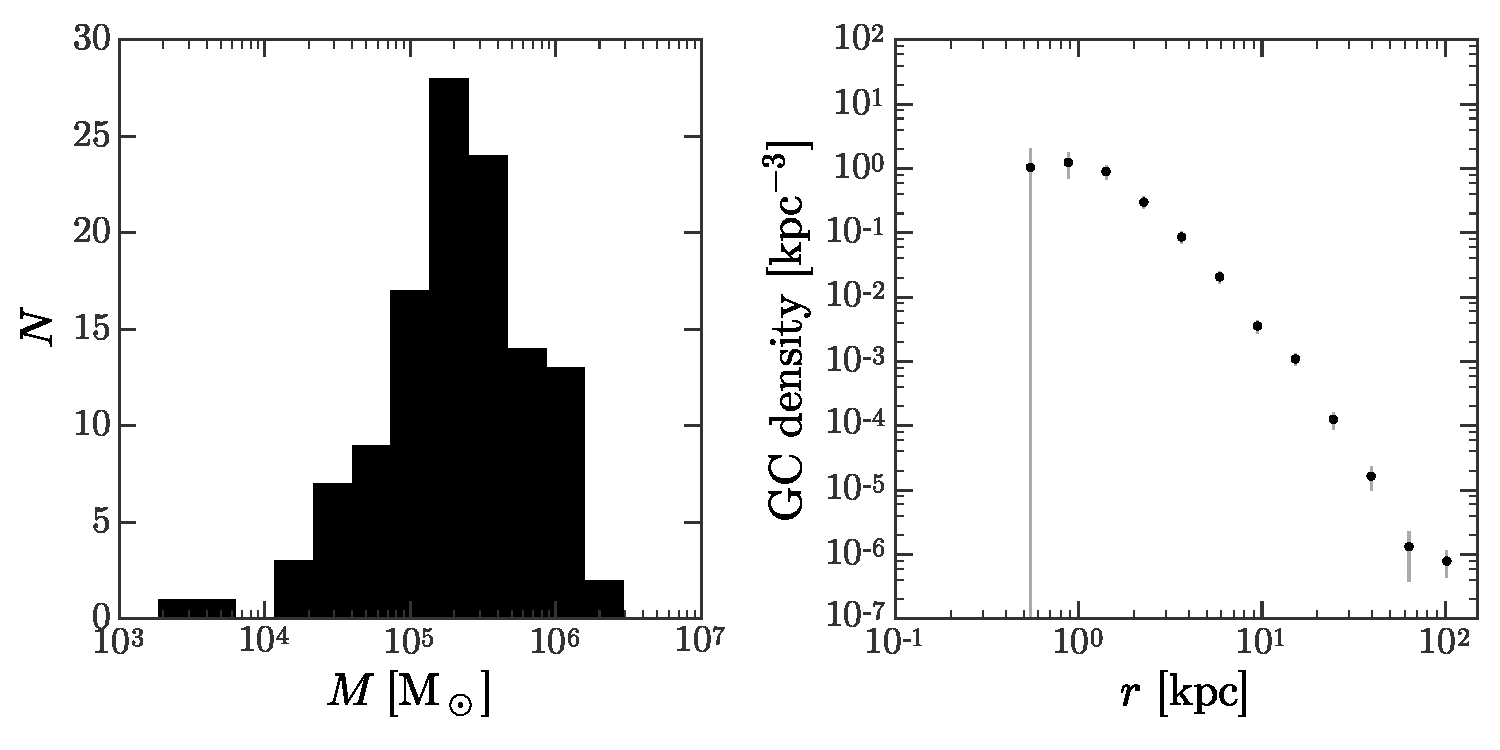
\includegraphics[width=\textwidth]{figures/mass-gcdensity.pdf}
\end{center}
\caption{%
\todo{caption}
\label{fig:mw-gc-pop}}
\end{figure*}

We consider two qualitatively different scenarios:
\begin{enumerate}
  \item The globular cluster system is in place around the Milky Way at redshift
    $z=3$ and simply evolves to present day, and
    % with orbits drawn from a spherical, isotropic distribution function (\df)
  \item The globular clusters are deposited into the Milky Way from
    cosmologically-accreted, tidally-disrupted satellite galaxies.
    % with orbits drawn from subhalo orbits in a cosmological simulation.
\end{enumerate}
For both cases, we require that the number and radial profile of surviving
clusters is consistent with the observed metal-poor GCs around the Milky Way.
In the subsections that follow, we describe the methods we use to simulate these
two scenarios.

% For scenario 3, we use orbits of subhalos drawn from the Aquarius simulations
% (\citealt{aquarius}) and set the number of GCs in each satellite using a $M_{\rm
% halo}$-$M_{\rm GC}$ scaling relation (\citealt{Harris:2015}). \todo{What?}
% With orbital initial conditions for the GCs (from the three scenarios above), a
% mass model for the Milky Way, and an initial mass function for the cluster
% masses we can evolve a given GC population forward to present day and compare
% the population of surviving clusters with that observed around the Milky Way.

\subsection{Milky Way mass model} \label{sec:massmodel}

For the gravitational potential of the Milky Way, we use a multi-component
mass-model consisting of a spherical Navarro-Frenk-White (NFW) dark matter halo
(H; \citealt{Navarro:1996}), a Miyamoto-Nagai disk (D; \citealt{Miyamoto:1975}),
and a sum of spherical Hernquist profiles (\citealt{Hernquist:1990}) to model
the mass distribution in the central Galaxy (bulge, B, and nucleus, N).
The detailed shape of the central mass distribution should not impact the orbits
of the halo clusters we are interested in.
The gravitational potential forms for these components are:
\begin{eqnarray}
  \Phi_{\rm H} &=& \frac{G \, M_{\rm H}}{r_{\rm H}} \, \frac{\ln{(1+r/r_{\rm H})}}{r/r_{\rm H}}
  \\
  \Phi_{\rm D} &=& -\frac{G \, M_{\rm D}}{\sqrt{R^2 + (R_{\rm D} + \sqrt{z^2 + z_{\rm D}^2})^2}}
  \\
  \Phi_{\rm B} &=& -\frac{G \, M_{\rm B}}{r + r_{\rm B}}
  \\
  \Phi_{\rm N} &=& -\frac{G \, M_{\rm N}}{r + r_{\rm N}} \quad .
\end{eqnarray}
This is a relatively simple model for the Milky Way potential, however at the
radii that we are most interested (i.e. in the halo) it is a reasonable model
given the vast uncertainties in the shape and profile of the halo.

At present-day ($z=0$), we set the potential parameters as follows.
We fix the Bulge and Disk parameters following \citealt{Bovy:2015}.
We fit for the halo mass, halo scale radius, nucleus mass, and nucleus scale
radius using standard nonlinear least-squares fitting with a compilation of
Milky Way enclosed-mass measurements (\citealt{Koposov:2010,Deason:2012,
Deason:2012a,Gibbons:2014,Kupper:2015,MORETODO}).
The best-fit or adopted parameter values are given in
\tblname~\ref{tbl:potential-params};
in \figname~\ref{fig:mass-profile}, we plot the mass enclosed as a function of
radii (thick line) and the enclosed-mass measurements used to fit for the free
potential parameters (points and error bars).

\begin{figure*}[h]
\begin{center}
\includegraphics[width=0.65\textwidth]{figures/mass-profile.pdf}
\end{center}
\caption{%
\todo{caption}
\todo{What's going on at small radii? Bug in Gala?}
\label{fig:mass-profile}}
\end{figure*}

\todo{possibly relevant paper: https://arxiv.org/pdf/astro-ph/0505594v3.pdf}
To evaluate the potential at a past time, we fix the form of the potential but
assume that the mass of the halo decreases exponentially with increasing
redshift (\citealt{TODO}), the mass of the combined disk, bulge, and nucleus
decreases linearly with lookback time (\citealt{TODO}), and the scale lengths of
the disk decrease \todo{how?} (\citealt{TODO}).
These assumed scalings...\todo{explain why}:
\begin{eqnarray}
  M_{\rm H}(z) &=& M_{\rm H}(0) \, e^{-z}
  \\
  M_{\rm D, B, N}(t) &=& M_{\rm D, B, N}(0) \, + \eta\,t
  \\
  R_{\rm D} &=& ...
  \\
  z_{\rm D} &=& ...
  \quad ,
\end{eqnarray}
where $t=0$ is present day and we evolve the clusters starting at $t_0 =
-XX~{\rm Gyr}$, $z_0 = 3$.

\begin{floattable}
\begin{deluxetable}{r l}
\tabletypesize{\footnotesize}
\caption{Parameters for the adopted Milky Way gravitational potential model at
present day ($z=0$) \label{tbl:potential-params}}

\tablehead{%
    \colhead{name} & \colhead{value}
}
\startdata
$M_{\rm H}$ & $4.51 \times 10^{11}~\msun$ \\
$r_{\rm H}$ & $13.2~\kpc$ \\
\hline
$M_{\rm D}$ & $6.8 \times 10^{10}~\msun$ \\
$R_{\rm D}$ & $3~\kpc$ \\
$z_{\rm D}$ & $280~\pc$ \\
\hline
$M_{\rm B}$ & $5 \times 10^{9}~\msun$ \\
$r_{\rm B}$ & $1~\kpc$ \\
\hline
$M_{\rm N}$ & $1.76 \times 10^{9}~\msun$ \\
$r_{\rm N}$ & $67.9~\pc$ \\
\enddata

\end{deluxetable}
\end{floattable}

\subsection{Globular cluster initial mass distribution} \label{sec:gcmassdist}

We assume that the initial cluster masses $m_0$ are drawn from a power-law
mass distribution (e.g., \citealt{Gnedin:2014}):
\begin{eqnarray}
  p(M_0) = A \, M_0^{-2}, \quad M_{\rm min} < M_0 < M_{\rm max},
\end{eqnarray}
where $M_{\rm min} = 10^4~\msun$, $M_{\rm max} = 10^7~\msun$, and $A$ is the
normalization constant.
The power-law exponent ($\beta = 2$) is consistent with observed young massive
star clusters in nearby galaxies (\citealt{TODO}).
The minimum mass scale is somewhat arbitrary, but we expect lower mass clusters
to disrupt very early and probably before they are tidally stripped from their
host systems.
The maximum mass scale is fixed to the fiducial value used in
\citealt{Gnedin:2014}.

\subsection{Cluster orbits} \label{sec:aqorbits}

The orbits of the individual clusters are either drawn from (1) a spherical,
isotropic distribution function embedded in the (instantaneous) background Milky
Way potential (\sectionname~\ref{sec:massmodel}) or (2) are assumed to be
accreted cosmologically in satellites and deposited into the Milky Way once the
satellites fully disrupt.

\subsubsection{Case 1: Embedded spherical distribution function} \label{sec:sphdf}

For this case, we follow previous work and assume the density profile of the
initial globular cluster system follows a S\'ersic profile with effective radius
$R_e=4$ and index $n_s = 2.2$ (see \sectionname~3 in \citealt{Gnedin:2014}).
This choice comes from assuming that, if the globular cluster system were in
place at an early time, the density profile of clusters, $\nu(r)$, likely
follows that of the stars (which is approximately S\'ersic).
We use this tracer density profile $\nu(r)$ and compute a spherically-averaged
version of the Milky Way mass model to evaluate the relative potential
$\Psi(r,t) = -\Phi(r,t)$ and use Eddington's formula
(\citealt{Eddington:1916,Binney:2008}) to evaluate the \df, $f(\mathcal{E})$,
along a grid of relative energies $\mathcal{E} = \Psi - \frac{1}{2}v^2$:
\begin{eqnarray}
  f(\mathcal{E}) &=& \frac{1}{\sqrt{8}\,\pi} \, \frac{\dd}{\dd \mathcal{E}}
    \int_0^\mathcal{E} \, \frac{\dd \Psi}{\sqrt{\mathcal{E} - \Psi}} \,
    \frac{\dd \nu}{\dd \Psi} \quad .
\end{eqnarray}
We use inverse-transform sampling to sample radii from the tracer density
profile $\nu(r)$, then use rejection-sampling (\citealt{vonneumann}) to sample
velocity magnitudes from the \df\ at each radius.
We convert radius and velocity magnitude to full-space position and velocity
assuming isotropy.

\subsubsection{Case 2: Cosmological orbits from the Aquarius simulations} \label{sec:cosmoorbits}

todo

\subsection{Mass evolution of the clusters} \label{sec:mockstreams}

Our goal is to produce mock stellar halos of stellar debris lost from the
globular clusters as they evolve along their orbits within the Milky Way.
All of the stars stripped from a given cluster will initially remain close to
the cluster and form coherent tidal tails, but older tidal debris will phase-mix
and form a smoother background distribution (e.g., \citealt{Helmi:1999}).
Our approach is to generate simulated stellar streams without running full
$N$-body simulations by using an approximate method for populating the tidal
tails that form around each cluster.
In recent years, significant effort has been devoted to developing such methods
to generate model stellar streams to compare with observed stream star
kinematics for, e.g., measuring the gravitational field of the Milky Way
(\citealt{Kupper:2012,Bonaca:2014,Gibbons:2014,Bovy:2014,Fardal:2015}).
These methods operate in a similar way:
Given the orbit and mass evolution of a progenitor system (e.g., globular
cluster), star particles are released from the Lagrange points of the satellite
with a spread in position and velocity set by the mass of the satellite (e.g.,
\citealt{Johnston:1999}) and some tunable scale parameters.
In this work, we use the parametrization of \citealt{Fardal:2015}, who fit the
release distribution parameters by comparing to full $N$-body simulations across
a range of mass and orbital parameters.

These methods accurately reproduce the mean tracks of the streams that form, but
the density of stars along the streams is determined by the mass-loss from the
progenitor system.
The mass evolution is typically assumed to be approximately linear with time so
that equal-mass star particles can be released from the Lagrange points at
regular time intervals (e.g., in sync with the integration of the progenitor
orbit).
In this work, we initially populate the stream particles using a constant
mass-loss rate, but separately solve for the cluster mass evolution to compute
the instantaneous mass-loss rate from the cluster at every time.
We then use this mass-loss rate to weight the model stream particle masses
to better capture the true density structure along each stream.

\subsection{Cluster mass evolution} \label{sec:gcmassevolution}

We solve for the mass evolution of a cluster given its initial mass and full
orbit using a semi-analytical method similar to that described in
\citet{Gnedin:2014} (hereafter G14).
G14 simultaneously solve for the mass and mean-radius evolution of ensembles
of globular clusters using analytic prescriptions for cluster mass-loss due to
evaporation ($t_{\rm iso}$), tidal stripping ($t_{\rm tid}$), and stellar
evolution ($t_{\rm se}$) and orbital radius evolution from dynamical friction
($t_{\rm df}$).
As we are mainly interested in the halo globular clusters, in this work we
neglect dynamical friction---the dynamical friction timescale for our maximum
mass cluster ($10^7~\msun$) at a Galactocentric distance of 10 kpc is much
longer than a Hubble time even for a moderately eccentric orbit.
We use these timescales (see also \eqname s~3--8 in \citealt{Gnedin:2014}) to
numerically integrate a simple differential equation for cluster mass $M$:
\begin{eqnarray}
  \frac{\dd M}{\dd t} &=& \, -\frac{M}{\min\left(t_{\rm iso}, t_{\rm tid}, t_{\rm se}\right)}
\end{eqnarray}
where the timescales are generally functions of both mass and mean orbital
radius.
This simple model for cluster mass evolution is approximate in many ways, but
perhaps the most severe assumption is that it ignores gravitational shocking of
clusters on eccentric orbits:
Each cluster is assumed to be on a circular orbit at the mean orbital radius
along its orbit.

For cases when a GC is accreted from a satellite galaxy, we first solve for
the mass-loss of the cluster within the satellite system up until it passes the
tidal radius.
At this point, we begin evolving the mass of the cluster in the tidal field of
the Milky Way instead.
When generating mock stellar streams for the GCs, we only consider stars that
are disrupted after the GC is stripped from its parent.

This simple procedure is only used to determine the mass-loss history of a given
cluster.

\section{Results 1: Coherent structures and thin streams}

Number of streams, distribution of lengths, mass in coherent structures?

\section{Results 2: Phase-mixed debris and kinematic substructure}

Solar neighborhood, Gaia volume + uncertainties

\section{Discussion}\label{sec:discussion}

Caveats:
\begin{itemize}
  \item Simple potential model - not cosmological, spherical halo, no
    substructure, no bar!
  \item Neglect stars deposited from dwarf galaxies - will dominate the stellar
    halo. We are imagining being able to distinguish these from GC stars using
    detailed abundances.
\end{itemize}

\section{Conclusions} \label{sec:conclusions}

Number of thin streams more consistent with X...

Compare kinematic clustering to chemical clustering to see how much chaos there
is, how much potential has evolved since majority disrupted

If similar, then amount of clumpiness tells you the initial population of GCs --
star formation in early universe, globular cluster populations in dwarf
galaxies, etc.

\acknowledgements
This research made use of
Astropy, a community-developed core Python package for Astronomy
\citep{Astropy-Collaboration:2013}.

\bibliographystyle{aasjournal}
\bibliography{mwgcs}

\end{document}
